\documentclass[10pt]{article}
\usepackage[margin=1in]{geometry}
\usepackage[T1]{fontenc}
\usepackage{lmodern}
\usepackage{amsmath,amssymb}
\usepackage{booktabs}
\usepackage{graphicx}
\usepackage{xcolor}
\usepackage{tikz}
\usetikzlibrary{positioning,arrows.meta,shapes.geometric,calc}
\usepackage[numbers,sort&compress]{natbib}
\usepackage[hidelinks]{hyperref}
\usepackage{microtype}

\definecolor{ro}{HTML}{0072B2}   % head-limited / the retrained head
\definecolor{rg}{HTML}{E69F00}   % representation-limited
\newcommand{\todo}[1]{\textcolor{red}{[TODO: #1]}}
% results still running: highlighted so none survives into the final version
\newcommand{\pend}[1]{\par\noindent\colorbox{yellow!45}{\parbox{\dimexpr\linewidth-2\fboxsep}{\footnotesize\textbf{PENDING:} #1}}\par}
\newcommand{\tbd}{\colorbox{yellow!45}{\strut ??}}
\newcommand{\hl}[1]{\textbf{#1}}   % head-limited cell
\setlength{\textfloatsep}{12pt plus 2pt minus 4pt}

\title{Head or Representation? Diagnosing Distribution-Shift Failures\\of Visuomotor Policies with Last-Layer Retraining}
\author{\todo{author}}
\date{}

\begin{document}
\maketitle

\begin{abstract}
Imitation-learned visuomotor policies often fail under distribution shift, but a success rate does
not tell whether the representation or the action head that reads it is at fault, and the two differ
greatly in the cost of a fix. We bring last-layer retraining from image
classifiers to closed-loop policies, retraining only the action head on states the policy visits. The
label is the frozen policy's own action on the same state rendered without the perturbation, which
simulation gives for free. We call a failure \emph{head-limited} if the retrained policy
beats both the base policy and an invisible-object negative control. Across ACT, Diffusion Policy and
SmolVLA, 9 of 11 visual failures on robomimic Lift are head-limited. In addition, for an object placed
out of range, retraining ACT's 5{,}130-weight head recovers over half of the gap with no
demonstrations. On Square and ToolHang, none of the 10 failures is head-limited, even when Square fails
only partly, and only fine-tuning below the head recovers success (25\% with LoRA, 43\% fully). Finally,
whether a linear probe decodes the grasp point does not predict which
failures the retrain fixes.
\end{abstract}

\section{Introduction}
\label{sec:intro}
Behavior-cloned visuomotor policies such as ACT~\citep{zhao2023act}, Diffusion
Policy~\citep{chi2023diffusion} and fine-tuned vision-language-action (VLA) models perform well in
distribution but fail just outside it. For example, they fail when the object sits a few centimeters
outside the demonstrated region or the camera is turned~\citep{xie2024decomposing,xue2025demogen,zhou2025liberopro}. If the policy's representation
still encodes what the task needs and only the action head fails to use it, a small change at the
output may be enough. If the representation itself breaks, the fix needs new data or retraining.
Linear probes can show that the information is present~\citep{lu2025probing,zhang2026probeact}, but
not that the policy can act on it.

We test this directly by freezing the backbone and retraining only the head
(Figure~\ref{fig:overview}). Image classification uses the same test to separate the quality of the
features from how the last layer weights them~\citep{kirichenko2023last,izmailov2022feature}. A policy,
however, acts in closed loop, where its errors compound, so we retrain it on the states it visits, as in
DAgger~\citep{ross2011dagger}. In addition, simulation gives exact labels for free. The same state can be
rendered with and without the perturbation~\citep{james2019rcan}, and the frozen policy's action on the
unperturbed render becomes the target, much as a privileged teacher relabels a
student~\citep{chen2019lbc}. If the retrain beats a policy that cannot see the object, the
representation was sufficient and the failure is \emph{head-limited}. Otherwise, it is
\emph{representation-limited}. Our contributions are threefold. (i) We bring last-layer retraining to
closed-loop policies as a diagnostic, with on-policy counterfactual labels, an invisible-object control
and an explicit decision rule, and apply it to ACT, Diffusion Policy and
SmolVLA~\citep{shukor2025smolvla}. (ii) We show that head-limited failures are common and that the
retrain then fixes them, including 9 of 11 visual failures on Lift and an out-of-range object.
(iii) We show that no failure is head-limited on the precise tasks, Square and ToolHang, even when the
policy fails only partly, so in our tasks the regime depends on the task more than on severity. A linear probe
of the grasp point does not predict the regime.

\begin{figure}[t]
\centering
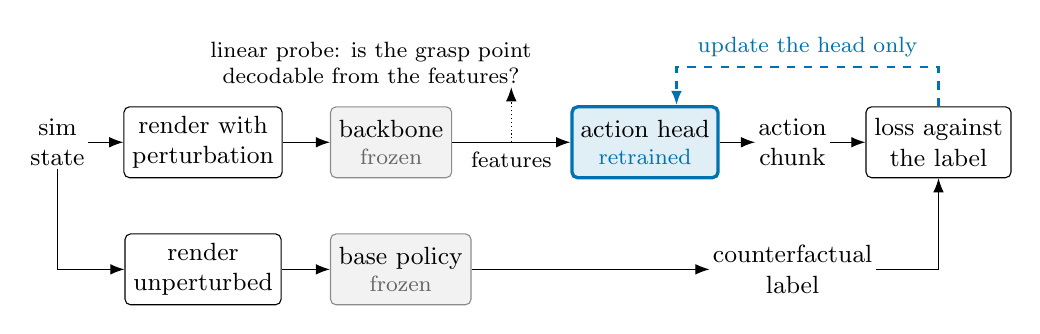
\begin{tikzpicture}[
  >={Latex[length=1.8mm]}, font=\small, node distance=4mm and 4.5mm,
  blk/.style={draw, rounded corners=2pt, align=center, minimum height=9mm, inner sep=3pt},
  frz/.style={blk, fill=black!5, draw=black!45},
  ed/.style={blk, fill=ro!12, draw=ro, very thick},
  txt/.style={align=center, inner sep=1pt},
  lbl/.style={font=\footnotesize, above, midway},
]
\node[txt] (s) {sim\\state};
\node[blk, right=of s] (rx) {render with\\perturbation};
\node[frz, right=6mm of rx] (enc) {backbone\\[-1pt]{\footnotesize\color{black!60} frozen}};
\node[ed, right=15mm of enc] (h) {action head\\[-1pt]{\footnotesize\color{ro} retrained}};
\node[txt, right=of h] (a) {action\\chunk};
\node[blk, right=of a] (L) {loss against\\the label};
\draw[->] (s) -- (rx);
\draw[->] (rx) -- (enc);
\draw[->] (enc) -- node[lbl, below]{features} (h);
\draw[->] (h) -- (a);
\draw[->] (a) -- (L);
\node[blk, below=7mm of rx] (r0) {render\\unperturbed};
\node[frz, anchor=west, minimum width=0pt] (pi0) at ($(enc.west |- r0)$)
  {base policy\\[-1pt]{\footnotesize\color{black!60} frozen}};
\node[txt] (y) at (a |- r0) {counterfactual\\label};
\draw[->] (s) |- (r0);
\draw[->] (r0) -- (pi0);
\draw[->] (pi0) -- (y);
\draw[->] (y) -| (L);
\draw[->, dashed, ro, thick] (L.north) -- ++(0,5mm) -| node[pos=0.25, above, font=\footnotesize]{update the head only} ([xshift=4mm]h.north);
\coordinate (gm) at ($(enc.east)!0.5!(h.west)$);
\node[txt, font=\footnotesize, anchor=south east] (P) at ($(gm)+(3mm,7mm)$) {linear probe: is the grasp point\\decodable from the features?};
\draw[->, densely dotted] (gm) -- (gm |- P.south);
\end{tikzpicture}
\caption{Last-layer retraining as a diagnostic. The frozen base policy's action on the unperturbed
render of the same state labels the head, the only part retrained. A linear probe is the comparison.}
\label{fig:overview}
\end{figure}

\paragraph{Related work.} Prior studies rank how visual factors and object placement hurt
imitation~\citep{xie2024decomposing,xue2025demogen}, and fine-tuned VLAs tend to replay memorized
trajectories~\citep{zhou2025liberopro}. Probes can find object states in VLA
layers~\citep{lu2025probing}, and ProbeAct uses a probe to correct a VLA's action at run
time~\citep{zhang2026probeact}. The closest work to ours is \citet{li2025vlagen}, who trace VLA failures
under visual perturbations to drift in the visual embedding and fix them by adapting the vision side
from one demonstration. In contrast, we retrain the output side, on three architectures and against a
negative control, and we also find failures that this retrain cannot fix. CFNBC~\citep{durso2026cfnbc}
uses paired counterfactual images to choose data for repair. In addition, encoders trained end to end
carry decision information~\citep{wang2024feature}, so a frozen backbone may not be enough. In
classifiers, the best layers to fine-tune depend on the kind of shift~\citep{lee2023surgical}. For our
policies, they depend on the task.

\section{Method}
\label{sec:method}
A policy maps image observations to an action chunk through a backbone and an action head. The head
is the last module through which the backbone's features reach the action. It is the linear action head
for ACT (5{,}130 of 52M weights), the FiLM layers that condition the denoiser for Diffusion Policy
(11.6M of 300M), and the action-expert output projection for SmolVLA (23{,}072 of 450M). A visual perturbation changes only how the simulator renders a
state and leaves the physics unchanged.

\paragraph{Step 1: retrain the head.} We roll out the base policy under the perturbation and label each
state it visits with the base policy's own action on the same state rendered without the perturbation.
We call this a \emph{counterfactual label}, and it requires no human and no demonstration. Object
position has no unperturbed render, so there we use two other sources of labels: an expert retrained on
shifted demonstrations and queried on the learner's states over two DAgger iterations, or
pseudo-labels that extend the policy's response from the nearest in-range position so that the action
follows the object fully. We then train only the head with the policy's own loss (for ACT's linear head, a
squared loss solved in closed form), adding in-distribution states labeled by the base policy to
preserve its behavior. For a visual perturbation, the whole budget is one
round of 30--60 perturbed and 20--30 in-distribution rollouts.

\emph{Negative control and decision rule.} When the object is rendered invisible (opacity 0), the
same retrain can at best learn to reach toward where the object usually is. Its success therefore
bounds what a retrain can gain without using the object. Let $[\ell, u]$ be the Wilson 95\% interval of
a success rate, for the base policy in distribution (in) and under the perturbation (base), the
retrained policy under the perturbation (ret), and the retrained control (ctl). Then
\begin{equation}
\text{failure:}\ u_\text{base} < \ell_\text{in}, \qquad
\text{head-limited:}\ \ell_\text{ret} > \max(u_\text{base},\, u_\text{ctl}),
\label{eq:rule}
\end{equation}
and a failure that is not head-limited is representation-limited.

\paragraph{Step 2: fine-tune deeper.} If the head retrain fails, we fine-tune LoRA~\citep{hu2022lora}
on every linear layer, and then the full network. We use the same kind of counterfactual labels,
collected over DAgger iterations~\citep{ross2011dagger}, each on the states of the latest fine-tuned
policy. The depth and number of iterations needed indicate how far below the head the failure sits.

\section{Setup}
\label{sec:setup}
We use the robomimic~\citep{mandlekar2021robomimic} tasks Lift, Square and ToolHang with
proficient-human demonstrations, in robosuite 1.4.1~\citep{zhu2020robosuite}, rendering ToolHang images
from its recorded states. All policies use two $84\times84$ cameras (agentview and wrist)
and absolute end-effector actions in chunks of 16. We train one ACT policy per task and one Diffusion
Policy each on Lift and Square, and we fine-tune SmolVLA on Lift. In distribution, success is 100\% on
Lift, 84\% (ACT) and 95\% (Diffusion Policy) on Square, and 46\% on ToolHang.

\emph{Perturbations} (Figure~\ref{fig:shifts}) apply to both cameras, because on Lift these policies
are robust to changes to a single camera. We use the agentview camera turned $30^\circ$ with the wrist
camera rolled $90^\circ$, a red table under dim light with the rolled wrist camera, both cameras upside
down, both cameras zoomed in, a faint object (opacity 0.1), and the invisible-object control. For
object position, we shift the Lift cube by $\pm5$ or $\pm7$\,cm along $x$ or $y$, on top of the
$\pm3$\,cm random placement in the demonstrations.
 We chose perturbation strengths on development seeds and collected labels on
training seeds, and we report closed-loop success on held-out test seeds.

\begin{figure}[t]
\centering
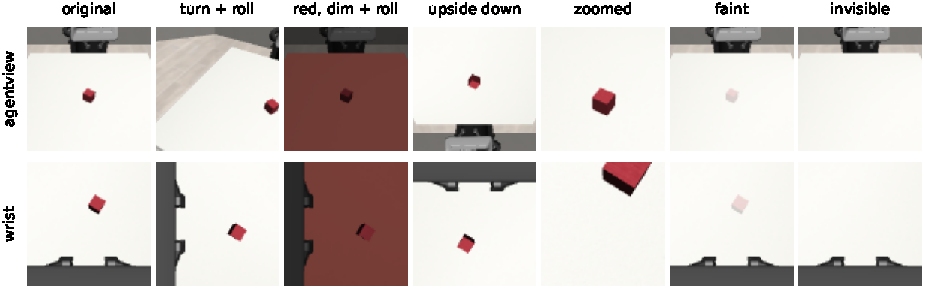
\includegraphics[width=0.46\linewidth]{figs/fig_shifts.pdf}
\caption{Visual perturbations on Lift, applied to both cameras. The invisible object is the control.}
\label{fig:shifts}
\end{figure}

\section{Results}
\label{sec:results}

\begin{table}[t]
\centering
\caption{Success (\%), base $\to$ head retrained (100 test episodes; 50 for SmolVLA and ToolHang;
$^\dagger$300). \hl{Bold}: head-limited; $^\circ$: not a failure. In distribution after the retrain:
98--100 on Lift, 70--90 (ACT) and 77--87 (Diffusion) on Square, 26--40 on ToolHang (base 46).}
\label{tab:grid}
\small
\setlength{\tabcolsep}{4pt}
\begin{tabular}{lcccccc}
\toprule
 & \multicolumn{3}{c}{Lift} & \multicolumn{2}{c}{Square} & ToolHang\\
\cmidrule(lr){2-4}\cmidrule(lr){5-6}\cmidrule(lr){7-7}
Perturbation & ACT & Diffusion & SmolVLA & ACT & Diffusion & ACT\\
\midrule
turn + roll      & 4 $\to$ 63$^\dagger$ & \hl{91 $\to$ 100} & \hl{64 $\to$ 88} & 0 $\to$ 0 & 1 $\to$ 2 & --\\
red, dim + roll  & \hl{49 $\to$ 78} & \hl{66 $\to$ 98}  & $90 \to 100^\circ$ & 2 $\to$ 0 & 0 $\to$ 1 & --\\
upside down      & \hl{36 $\to$ 85} & \hl{54 $\to$ 99}  & 56 $\to$ 72  & 0 $\to$ 1 & 0 $\to$ 1 & 0 $\to$ 0\\
zoomed           & \hl{37 $\to$ 83} & --           & --           & 0 $\to$ 0 & -- & --\\
faint            & \hl{82 $\to$ 100}& \hl{62 $\to$ 94}  & $90 \to 98^\circ$ & 2 $\to$ 1 & 0 $\to$ 0 & --\\
\midrule
invisible (control) & 28 $\to$ 55$^\dagger$ & 58 $\to$ 78 & 26 $\to$ 60 & 0 $\to$ 0 & 0 $\to$ 0 & 0 $\to$ 0\\
\midrule
head-limited / failures & 4/5 & 4/4 & 1/2 & 0/5 & 0/4 & 0/1\\
\bottomrule
\end{tabular}
\end{table}

\begin{table}[t]
\centering
\caption{Object position on Lift: success (\%), cube shifted $\pm5$/$\pm7$\,cm per axis (ACT 160 episodes
per axis, SmolVLA 120). ``Per axis'': one retrain per axis, scored on that axis.}
\label{tab:position}
\small
\begin{tabular}{llrrrr}
\toprule
Policy & Model & $x$ & $y$ & in-dist. & weights changed\\
\midrule
ACT & base & 55 & 47 & 100 & --\\
 & full retrain, 400 shifted demos (per axis) & 100 & 100 & 100 & 52M\\
 & head retrain, DAgger expert labels (per axis) & 99 & 91 & 100 & 5{,}130\\
 & head retrain, pseudo-labels, no demos & 85 & 72 & 99 & 5{,}130\\
 & head retrain, in-distribution labels (control) & 54 & 49 & 100 & 5{,}220\\
\midrule
SmolVLA & base & 67 & 46 & 100 & --\\
 & head retrain, DAgger expert labels (per axis) & 91 & 86 & 100 & 23{,}072\\
\bottomrule
\end{tabular}
\end{table}

\paragraph{Visual perturbations.} On Lift, 9 of the 11 perturbations that cause a failure are
head-limited, across all three policies, and in-distribution success stays intact
(Table~\ref{tab:grid}). The two exceptions recover no further than the blind control. They are ACT
under turn + roll (4\% $\to$ 63\%, control 55\%) and SmolVLA upside down (56\% $\to$ 72\%, control
60\%). For ACT, the control succeeds on 69\% of placements near the center and 40\% of those
farther away, as a reach that ignores the cube would. Two verdicts clear the bar by less than 1.5 points (Diffusion Policy and SmolVLA under
turn + roll). On Square and ToolHang, none of the 10 failures is head-limited. The retrain leaves every
policy at 0--2\% and costs up to 20 points in distribution.

\paragraph{Task or severity?} Table~\ref{tab:grid} confounds the task with the severity of the failure,
since the same perturbations drop Square to 0--2\%. We therefore weakened the perturbations on Square
until the policies fail only partly. A less faint object does this for both policies, and a wrist roll
alone does it for Diffusion Policy, while camera changes drive ACT to 0\% even at a $10^\circ$ turn.
None of these partial failures is head-limited. At object opacity 0.3, ACT goes from 36\% to 51\% and
Diffusion Policy from 24\% to 26\%, and with the wrist camera rolled, Diffusion Policy goes from 28\% to
41\%. Each retrained interval overlaps the base policy's. With the policy and the type of
perturbation fixed, a faint object takes Diffusion Policy from
62\% to 94\% on Lift but only from 24\% to 26\% on Square, even though the Square object is less faint
(opacity 0.3 vs.\ 0.1). In our tasks, the regime depends on the task more than on the severity. However, severity still matters within Lift, as ACT's turn + roll exception shows.

\paragraph{Object position.} When the cube is out of range, a probe at ACT's head input still follows
the cube's offset, with a gain of 0.85 and 0.78 per unit offset in $x$ and $y$ (by finite
differences), while the action barely follows it (0.28 and 0.09). Using in-range feature directions at
out-of-range states, a first-order interchange intervention~\citep{geiger2021causal} restores the gain
(0.66 and 0.65), so the offset moves the features in directions the head never learned to read. Retraining the 5{,}130-weight head on pseudo-labels, with no demonstrations,
recovers over half of the gap (Table~\ref{tab:position}). With labels from the 400-demonstration
retrain, the head retrain nearly matches that retrain, partly through distillation. Retraining on
in-distribution labels alone, which serves as the control here, has no effect, so the failure is
head-limited and the gain comes from the labels. SmolVLA, with labels from the same ACT expert, is
fixed in the same way, although its $y$ retrain lowers its $x$ success from 67\% to 55\%.

\paragraph{The probe does not predict the regime.} We fit a ridge probe from the head's input features to the grasp
point (the table position of the cube, nut handle or tool) on frames before contact, and score it by $R^2$ cross-validated across episodes. In distribution, the probe decodes the
grasp point on Lift and Square ($R^2$ 0.78--0.93) but not on ToolHang (0.25), where the tool moves by
only 11\,mm. When fit jointly on in-distribution and perturbed features, ACT's probe
keeps the grasp point on Lift (0.39--0.90) and loses it on Square ($-0.22$ and $-0.23$ for the two
perturbations we probed). However, Diffusion Policy upside down on Lift is fixed even though its $R^2$
is 0.20, while ACT under turn + roll (0.85) and the partial Square failures (0.18--0.49) are not.

\paragraph{Square needs depth.} For ACT on Square under turn + roll, full fine-tuning (Step~2) scores 0, 1,
18, 43 and 40\% over DAgger iterations 1--5, although the first round already brings the gripper from
210\,mm to 53\,mm of the handle. With the same four iterations of labels, the head
alone stays at 0\%, LoRA (rank 8, 457K weights) reaches 25\%, and full fine-tuning reaches 43\% (the
iterations followed the fully fine-tuned policy, which favors it). In-distribution success drops from 84\% to 73\% after four iterations and to 48\% after five.
ToolHang stays out of reach, with 0 of 30 successes after two iterations and 0 of 30 in distribution.

\section{Conclusion and limitations}
\label{sec:conclusion}
A head retrain on free counterfactual labels, compared against an invisible-object control, sorts
distribution-shift failures into the two regimes after one round of rollouts, and when a failure is
head-limited, the retrain is already the fix. The labels are exact only in
simulation, but run in simulation or a digital twin under the changes a deployment expects, the
diagnosis tells in advance whether a failure needs only a head retrain or new data and deeper training. On a real robot, a fixed reference camera gives exact labels for a camera
change, and image editing or human corrections can approximate them otherwise.

\emph{Limitations.} We have no real-robot results, and our position expert needed 400 shifted
demonstrations. Each configuration is one trained policy, scored on 50--300 episodes. The two precise
tasks also have lower in-distribution success, which limits what counterfactual labels can teach. The head is chosen per architecture, and for
Diffusion Policy it is large. We tested ToolHang under one perturbation and Step~2 on ACT only.

\bibliographystyle{unsrtnat}
\bibliography{refs}
\end{document}
